
    \begin{figure}[t]
        \hspace{-10pt}
        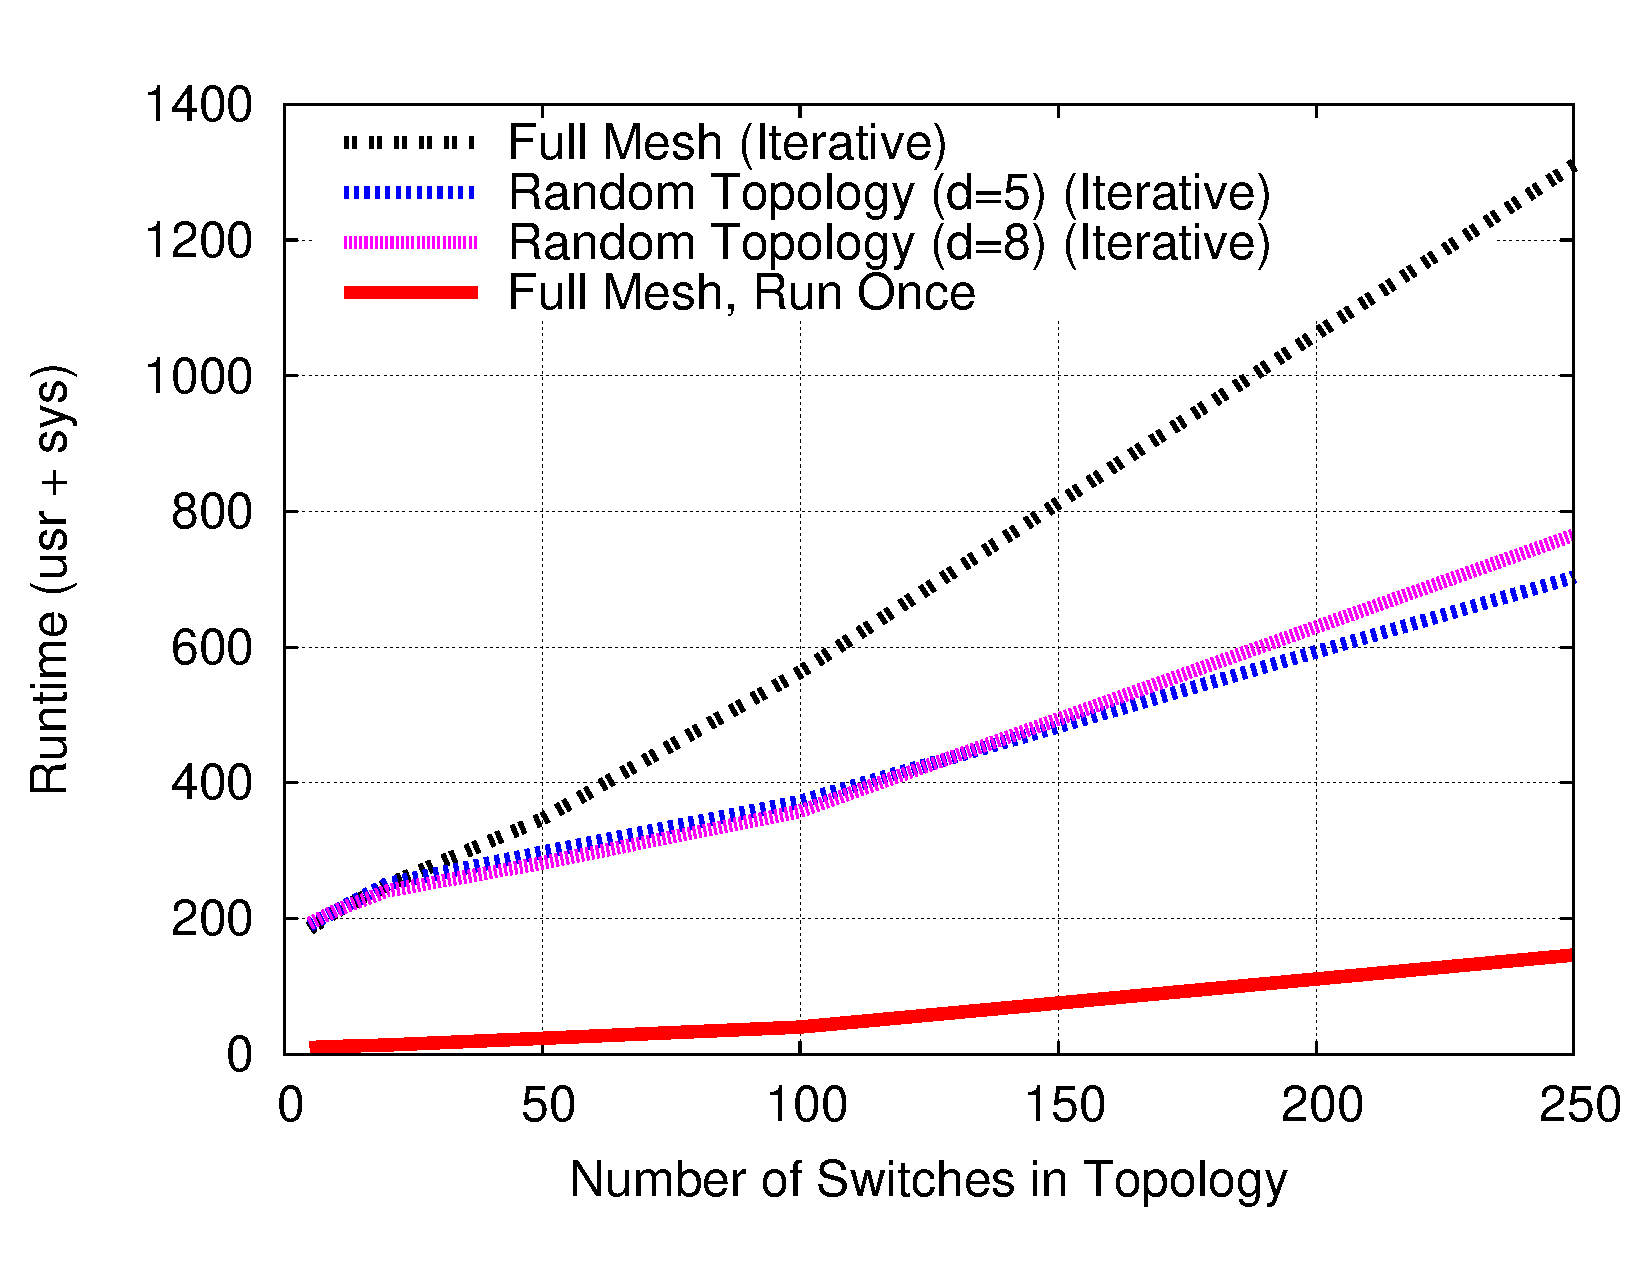
\includegraphics[width=3.25in]{graph}
        \caption[]{\label{fig:anteatertime} Execution time to run invariant checker over full mesh and randomly generated network topologies of 5 to 250 nodes.} 
    \end{figure}



    We are building an implementation of CLINT to debug SDN networks running the POX network operating system~\cite{pox}.
    
    POX is an implementation of the NOX network operating system built in Python.
    POX applications are typically written for a single controller with only minimal virtualization.
    To study \projectname{}'s ability to capture virtualization errors, we extended POX
    to support a simple virtualization layer that presents switches as Python objects to the control application.
    The virtualization layer does not yet support more complex virtualization such as `big switch' representations 
    of the network; in future work we plan to extend it to so.
    To study bugs that arise between replicated controllers, we also extended POX to support replicated controllers
    with eventually-consistent shared state.

    The current implementation of CLINT supports two features outlined in \S\ref{sec:architecture}, a traffic and topology `fuzzer' for input generation, and an invariant checker to detect bugs that manifest in the physical network.
    Our invariant checker is an extension of the Anteater~\cite{anteater} network debugger.
    In future work, we plan to develop a correspondence checker to do cross-layer and cross-controller analysis over the improved version of POX that we developed this semester.
    
    \projectname{}'s physical network invariant checker is an extended deployment of Anteater~\cite{anteater}, which is extensively evaluated in the Anteater paper.
    Anteater is capable of detecting loops, dead-ends, network partitions, and consistency violations.
    Our modifications to Anteater include adapting it to check FIB entries from a simulated network run under POX and integrating it with our input generator to run Anteater iteratively.
   
    We evaluated the performance of our iteratively run invariant checks by running our implementation over various network topologies with sizes scaling from five switches to 250, a full mesh network (with each node connected to $n - 1$ other nodes), and a randomly generated topology with each node randomly connected to 5 or 8 other nodes.
    We ran the invariant checker with rounds of 100 inputs from the input generator, with invariant checks run after every fifth input (for a total of 20 runs of the invariant checker).
    The time for the invariant checker to evaluate the network is plotted in Figure~\ref{fig:anteatertime}.
   
    \justine{Colin, can you bullshit something here? I have no idea what to say.} 

    \subsection{Next Steps}
        The previously described experiments show that our implementation of \projectname{} (1) can detect errors like forwarding loops that manifest entirely in the physical network (by using Anteater), (2) can detect physical network errors that manifest as the result of a specific sequence of flows to reach the network controller (by using \projectname{}'s network fuzzer), and (3) imposes reasonable performance requirements to analyze the SDN stack for these errors.
        To complete this analysis, we are working with engineers at Nicira Networks to obtain in-depth bug reports describing errors encountered by real SDN deployments.
        In future work, we plan to replicate these bugs in our SDN testbed and investigate whether \projectname{} can detect them.
        In addition, we are working with researchers at the International Computer Science Institute (ICSI) to obtain copies of their own SDN control applications from their research, and apply \projectname{} to their implementations to investigate whether \projectname{} can detect any new bugs.

        Longer term, as the \projectname{} implementation matures to include multi-layer correspondence checks and cross-controller consistency checks (as described in \S\ref{sec:architecture}), we will apply \projectname{} to a broader class of bugs and see what fraction of Nicira bug reports \projectname{} can capture, and what kinds of new bugs it detects in control applications from ICSI. 


